\documentclass[tikz,border=3.14mm]{standalone}
\usetikzlibrary{arrows.meta, positioning}

\begin{document}
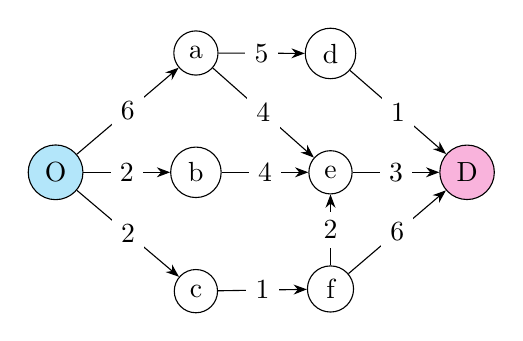
\begin{tikzpicture}[>=Stealth, node distance=0.9cm and 1.1cm]
    \node (O) [draw, circle, fill=cyan!30] {O};
    \node (b) [right=of O, draw, circle] {b};
    \node (e) [right=of b, draw, circle] {e};
    \node (D) [right=of e, draw, circle, fill=magenta!30] {D};
    \node (a) [above=of b, draw, circle] {a};
    \node (c) [below=of b, draw, circle] {c};
    \node (d) [above=of e, draw, circle] {d};
    \node (f) [below=of e, draw, circle] {f};

    % Edges with weights
    \draw[->] (O) -- node[label, midway, fill=white]{2} (b);
    \draw[->] (b) -- node[midway, fill=white]{4} (e);
    \draw[->] (e) -- node[midway, fill=white]{3} (D);
    \draw[->] (O) -- node[midway, fill=white]{6} (a);
    \draw[->] (a) -- node[midway, fill=white]{5} (d);
    \draw[->] (d) -- node[midway, fill=white]{1} (D);
    \draw[->] (a) -- node[midway, fill=white]{4} (e);
    \draw[->] (O) -- node[label, midway, fill=white]{2} (c);
    \draw[->] (c) -- node[label, midway, fill=white]{1} (f);
    \draw[->] (f) -- node[label, midway, fill=white]{2} (e);
    \draw[->] (f) -- node[label, midway, fill=white]{6} (D);
\end{tikzpicture}
\end{document}